\section{User Interface} \label{sec:UserInterface}
The user interface module, shown on figure \refq{fig_6_5_UserInterface}, is a touchscreen that the user can use to set the test parameters for the DUT. The screen will display the test results to the user in whichever format the user has choser, either numerically or with a graph.

\begin{figure}[H]
    \centering
    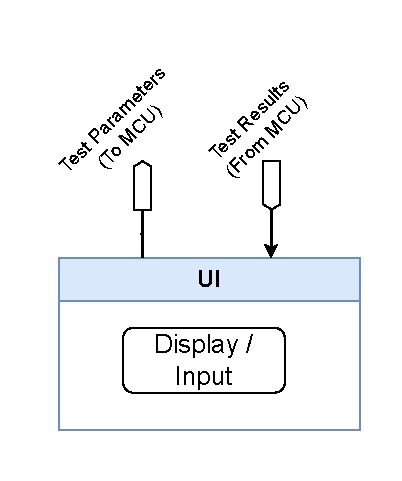
\includegraphics[clip, trim=18 0 18 0,width=0.40\textwidth]{Sections/6_SystemArchitecture/Figures/UI.pdf}
    \caption{The user interface is a touchscreen. The user can set the test parameters for the DUT and the display can show the results.}
    \label{fig_6_5_UserInterface}
\end{figure}

The \textit{user interface} module is also a USB device that the user can use to retrieve test results from the instrument. It is envisioned that the user can start a transfer from the impedance analyzer and the instrument will then proceed to dump all the test results in a string of comma separated values over the serial connection. It will be up to the user to \textit{listen in} and log the results from a serial monitor such as puTTY, or similar.
